% Practice Test 05 — Indiana Edition
% Questions: 30 (25 MC + 5 SA)
% Generated by scripts/generate_practice_tests.py

\begin{practiceQuestion}{1-3-q04}{mc}
\begin{questionText}
Bananas cost a fixed price per pound. The table shows the relationship. What is $k$?

\begin{center}
\begin{tabular}{|c|c|}
\hline \textbf{Pounds} & \textbf{Cost (\$)} \\ \hline $2$ & $\$1.30$ \\ $5$ & $\$3.25$ \\ $8$ & $\$5.20$ \\ \hline
\end{tabular}
\end{center}
\end{questionText}
\choiceA{$\$0.55$ per pound}
\choiceB{$\$0.65$ per pound}
\choiceC{$\$1.30$ per pound}
\choiceD{$\$1.54$ per pound}
\correctAnswer{B}
\explanation{$k = \frac{1.30}{2} = 0.65$. Check: $\frac{3.25}{5} = 0.65$ and $\frac{5.20}{8} = 0.65$. Bananas cost $\$0.65$ per pound.}
\end{practiceQuestion}

\begin{practiceQuestion}{1-5-q15}{mc}
\begin{questionText}
The slope of a proportional line is $\frac{7}{2}$. What is the unit rate?
\end{questionText}
\choiceA{$2$}
\choiceB{$3.5$}
\choiceC{$7$}
\choiceD{$14$}
\correctAnswer{B}
\explanation{For proportional relationships, slope $= k =$ unit rate. $\frac{7}{2} = 3.5$.}
\end{practiceQuestion}

\begin{practiceQuestion}{1-6-q06}{mc}
\begin{questionText}
Small paint can: $\frac{3}{4}$ gallon for $\$18$. Large can: $1\frac{1}{2}$ gallons for $\$33$. Which is the better buy?
\end{questionText}
\choiceA{Small, at $\$22$/gal}
\choiceB{Large, at $\$22$/gal}
\choiceC{Small, at $\$24$/gal}
\choiceD{Large, at $\$24$/gal}
\correctAnswer{B}
\explanation{Small: $18 \div 0.75 = \$24$/gal. Large: $33 \div 1.5 = \$22$/gal. The large can is $\$2$/gal cheaper.}
\end{practiceQuestion}

\begin{practiceQuestion}{2-2-q24}{sa}
\begin{questionText}
$156$ is $120\%$ of what number?
\end{questionText}
\correctAnswer{$130$}
\explanation{$\frac{156}{w} = \frac{120}{100}$. Cross-multiply: $120w = 15{,}600$. Divide: $w = 130$.}
\end{practiceQuestion}

\begin{practiceQuestion}{2-5-q27}{gmc}
\begin{questionText}
The bar graph shows the tip amounts left by four customers at a restaurant where all bills were $\$60$. Which customer left approximately a $20\%$ tip?

\begin{center}
\begin{tikzpicture}[scale=0.55]
  \draw[thick,->] (0,0) -- (0,5.5) node[above]{\small Tip (\$)};
  \draw[thick,->] (0,0) -- (8,0);
  \fill[funBlue!60] (0.5,0) rectangle (1.5,2.7);
  \fill[funGreen!60] (2.5,0) rectangle (3.5,4);
  \fill[funOrange!60] (4.5,0) rectangle (5.5,3);
  \fill[funRed!60] (6.5,0) rectangle (7.5,1.5);
  \node[below,font=\small] at (1,0) {A};
  \node[below,font=\small] at (3,0) {B};
  \node[below,font=\small] at (5,0) {C};
  \node[below,font=\small] at (7,0) {D};
  \foreach \y/\lab in {1/3,2/6,3/9,4/12,5/15} {
    \draw (-0.1,\y) -- (0.1,\y) node[left,font=\small,xshift=-2pt] {\lab};
  }
  \node[above,font=\small] at (1,2.7) {$\$8$};
  \node[above,font=\small] at (3,4) {$\$12$};
  \node[above,font=\small] at (5,3) {$\$9$};
  \node[above,font=\small] at (7,1.5) {$\$5$};
\end{tikzpicture}
\end{center}
\end{questionText}
\choiceA{Customer A}
\choiceB{Customer B}
\choiceC{Customer C}
\choiceD{Customer D}
\correctAnswer{B}
\explanation{$20\%$ of $\$60 = \$12$. Customer B left $\$12$, which is exactly $20\%$.}
\end{practiceQuestion}

\begin{practiceQuestion}{2-7-q16}{mc}
\begin{questionText}
An estimate has a percent error of $0\%$. What does this mean?
\end{questionText}
\choiceA{The estimate was very close}
\choiceB{The estimate was exactly correct}
\choiceC{The actual value was $0$}
\choiceD{There was no actual value to compare}
\correctAnswer{B}
\explanation{A $0\%$ percent error means the estimated value equals the actual value exactly.}
\end{practiceQuestion}

\begin{practiceQuestion}{3-1-q10}{mc}
\begin{questionText}
A football team gains $8$ yards on one play and loses $8$ yards on the next play. What is the net result?
\end{questionText}
\choiceA{$16$ yards gained}
\choiceB{$8$ yards gained}
\choiceC{$8$ yards lost}
\choiceD{$0$ yards}
\correctAnswer{D}
\explanation{$8 + (-8) = 0$. Gaining and losing the same amount are opposite actions that cancel out.}
\end{practiceQuestion}

\begin{practiceQuestion}{3-2-q28}{gmc}
\begin{questionText}
Look at the table of deposits and withdrawals from a bank account.

\begin{center}
\begin{tabular}{|c|c|}
\hline
\textbf{Day} & \textbf{Transaction} \\
\hline
Monday & $+\$30$ \\
\hline
Tuesday & $-\$45$ \\
\hline
Wednesday & $+\$20$ \\
\hline
Thursday & $-\$15$ \\
\hline
\end{tabular}
\end{center}

If the account started at $\$0$, what is the balance after Thursday?
\end{questionText}
\choiceA{$\$110$}
\choiceB{$-\$10$}
\choiceC{$\$10$}
\choiceD{$-\$50$}
\correctAnswer{B}
\explanation{$0 + 30 + (-45) + 20 + (-15) = 30 + 20 - 45 - 15 = 50 - 60 = -10$. The balance is $-\$10$.}
\end{practiceQuestion}

\begin{practiceQuestion}{4-2-q13}{mc}
\begin{questionText}
Which expression is already simplified (cannot be combined further)?
\end{questionText}
\choiceA{$4x + 3x$}
\choiceB{$5a - 2a + 7$}
\choiceC{$3m + 8$}
\choiceD{$6 + 9 - 2$}
\correctAnswer{C}
\explanation{$3m + 8$ has no like terms to combine ($3m$ is a variable term and $8$ is a constant). The others can all be simplified further.}
\end{practiceQuestion}

\begin{practiceQuestion}{4-3-q01}{mc}
\begin{questionText}
Expand $3(x + 4)$.
\end{questionText}
\choiceA{$3x + 4$}
\choiceB{$3x + 12$}
\choiceC{$3x + 7$}
\choiceD{$12x$}
\correctAnswer{B}
\explanation{Multiply $3$ by each term: $3 \times x = 3x$ and $3 \times 4 = 12$. Result: $3x + 12$.}
\end{practiceQuestion}

\begin{practiceQuestion}{5-4-q03}{mc}
\begin{questionText}
Solve $0.25n - 1.5 = 3.5$.
\end{questionText}
\choiceA{$n = 8$}
\choiceB{$n = 20$}
\choiceC{$n = 14$}
\choiceD{$n = 2$}
\correctAnswer{B}
\explanation{Add $1.5$: $0.25n = 5$. Divide by $0.25$: $n = 20$. Check: $0.25(20) - 1.5 = 5 - 1.5 = 3.5$ \checkmark.}
\end{practiceQuestion}

\begin{practiceQuestion}{5-5-q08}{mc}
\begin{questionText}
Solve $\dfrac{x}{3} + 4 < 10$.
\end{questionText}
\choiceA{$x < 18$}
\choiceB{$x < 42$}
\choiceC{$x < 2$}
\choiceD{$x < 6$}
\correctAnswer{A}
\explanation{Subtract $4$: $\frac{x}{3} < 6$. Multiply by $3$: $x < 18$.}
\end{practiceQuestion}

\begin{practiceQuestion}{5-6-q18}{mc}
\begin{questionText}
Solve $6 - 2x \leq -4$ and describe the graph.
\end{questionText}
\choiceA{Closed circle at $5$, shade right}
\choiceB{Open circle at $5$, shade right}
\choiceC{Closed circle at $5$, shade left}
\choiceD{Closed circle at $-5$, shade right}
\correctAnswer{A}
\explanation{Subtract $6$: $-2x \leq -10$. Divide by $-2$ and flip: $x \geq 5$. Closed circle at $5$, shade right.}
\end{practiceQuestion}

\begin{practiceQuestion}{6-1-q29}{gsa}
\begin{questionText}
The scale drawing below shows an L-shaped room. The scale is $1$ cm $= 2$ m. What is the actual area of the room?

\begin{center}
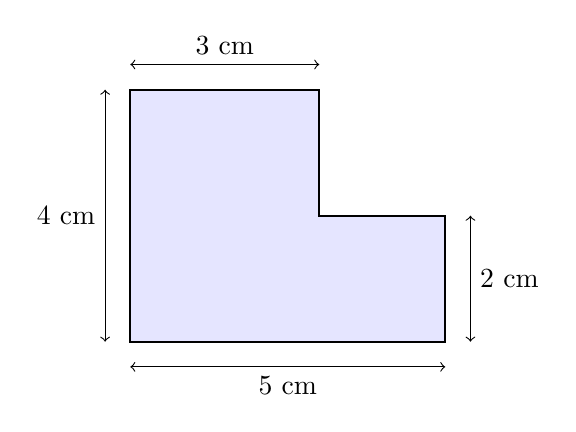
\begin{tikzpicture}[scale=0.8]
  \draw[thick,fill=blue!10] (0,0) -- (5,0) -- (5,2) -- (3,2) -- (3,4) -- (0,4) -- cycle;
  \draw[<->] (0,-0.4) -- (5,-0.4);
  \node[below] at (2.5,-0.4) {$5$ cm};
  \draw[<->] (5.4,0) -- (5.4,2);
  \node[right] at (5.4,1) {$2$ cm};
  \draw[<->] (-0.4,0) -- (-0.4,4);
  \node[left] at (-0.4,2) {$4$ cm};
  \draw[<->] (0,4.4) -- (3,4.4);
  \node[above] at (1.5,4.4) {$3$ cm};
\end{tikzpicture}
\end{center}
\end{questionText}
\correctAnswer{$64$ m$^2$}
\explanation{Split into two rectangles. Left: $3$ cm $\times$ $4$ cm $= 12$ cm$^2$. Bottom-right: $(5-3)$ cm $\times$ $2$ cm $= 4$ cm$^2$. Total drawing area: $16$ cm$^2$. Scale: $1$ cm $= 2$ m, so areas scale by $2^2 = 4$. Actual area: $16 \times 4 = 64$ m$^2$.}
\end{practiceQuestion}

\begin{practiceQuestion}{6-3-q17}{mc}
\begin{questionText}
A triangle has side lengths $9$, $12$, and $15$. What type of triangle is it?
\end{questionText}
\choiceA{Equilateral}
\choiceB{Isosceles}
\choiceC{Right}
\choiceD{It cannot be formed}
\correctAnswer{C}
\explanation{Check: $9^2 + 12^2 = 81 + 144 = 225 = 15^2$. Since the Pythagorean theorem holds, this is a right triangle.}
\end{practiceQuestion}

\begin{practiceQuestion}{6-4-q08}{mc}
\begin{questionText}
You know two angles ($50°$ and $70°$) and the side between them is $8$ cm. What triangle condition is this?
\end{questionText}
\choiceA{SSS}
\choiceB{SAS}
\choiceC{ASA}
\choiceD{AAS}
\correctAnswer{C}
\explanation{Two angles and the included side is the ASA (Angle-Side-Angle) condition.}
\end{practiceQuestion}

\begin{practiceQuestion}{6-5-q08}{mc}
\begin{questionText}
A cylinder is sliced with a vertical cut through its center, perpendicular to the base. What shape is the cross-section?
\end{questionText}
\choiceA{Circle}
\choiceB{Rectangle}
\choiceC{Oval}
\choiceD{Triangle}
\correctAnswer{B}
\explanation{A vertical cut through the center of a cylinder produces a rectangle. The width equals the diameter and the height equals the cylinder's height.}
\end{practiceQuestion}

\begin{practiceQuestion}{6-6-q25}{sa}
\begin{questionText}
Two lines intersect. One of the four angles is $(4x + 20)°$. Its adjacent angle is $(6x - 10)°$. Find the value of $x$.
\end{questionText}
\correctAnswer{$17$}
\explanation{Adjacent angles at an intersection are supplementary: $4x + 20 + 6x - 10 = 180$. Combine: $10x + 10 = 180$. Solve: $10x = 170$, $x = 17$.}
\end{practiceQuestion}

\begin{practiceQuestion}{6-7-q02}{mc}
\begin{questionText}
Point $B(-2, 4)$ is reflected over the $x$-axis. What are the coordinates of $B'$?
\end{questionText}
\choiceA{$(-2, -4)$}
\choiceB{$(2, 4)$}
\choiceC{$(2, -4)$}
\choiceD{$(-2, 4)$}
\correctAnswer{A}
\explanation{Reflection over the $x$-axis: keep $x$, negate $y$. $(-2, 4) \to (-2, -4)$.}
\end{practiceQuestion}

\begin{practiceQuestion}{7-3-q10}{mc}
\begin{questionText}
A semicircle has a radius of $6$ inches. What is the area of the semicircle? Use $\pi \approx 3.14$.
\end{questionText}
\choiceA{$18.84$ in$^2$}
\choiceB{$56.52$ in$^2$}
\choiceC{$113.04$ in$^2$}
\choiceD{$37.68$ in$^2$}
\correctAnswer{B}
\explanation{Full circle area $= \pi r^2 = 3.14 \times 36 = 113.04$ in$^2$. Semicircle $= 113.04 \div 2 = 56.52$ in$^2$.}
\end{practiceQuestion}

\begin{practiceQuestion}{7-4-q10}{mc}
\begin{questionText}
A figure is made of a trapezoid with parallel sides $6$ cm and $10$ cm, and height $4$ cm. Which expression gives its area?
\end{questionText}
\choiceA{$6 \times 10 \times 4$}
\choiceB{$\frac{1}{2} \times 6 \times 10$}
\choiceC{$\frac{1}{2} \times (6 + 10) \times 4$}
\choiceD{$(6 + 10) \times 4$}
\correctAnswer{C}
\explanation{Area of a trapezoid $= \frac{1}{2}(b_1 + b_2) \times h = \frac{1}{2}(6 + 10) \times 4 = 32$ cm$^2$.}
\end{practiceQuestion}

\begin{practiceQuestion}{7-5-q18}{mc}
\begin{questionText}
A rectangular prism has a surface area of $94$ cm$^2$. Its length is $5$ cm and width is $3$ cm. What is its height?
\end{questionText}
\choiceA{$2$ cm}
\choiceB{$3$ cm}
\choiceC{$4$ cm}
\choiceD{$5$ cm}
\correctAnswer{C}
\explanation{$94 = 2(5 \times 3) + 2(5 \times h) + 2(3 \times h) = 30 + 10h + 6h = 30 + 16h$. So $16h = 64$, $h = 4$ cm.}
\end{practiceQuestion}

\begin{practiceQuestion}{7-6-q11}{mc}
\begin{questionText}
A triangular prism has a triangular base with legs $5$ cm and $12$ cm (right triangle). The prism is $15$ cm long. What is the volume?
\end{questionText}
\choiceA{$150$ cm$^3$}
\choiceB{$300$ cm$^3$}
\choiceC{$450$ cm$^3$}
\choiceD{$900$ cm$^3$}
\correctAnswer{C}
\explanation{$B = \frac{1}{2} \times 5 \times 12 = 30$ cm$^2$. $V = 30 \times 15 = 450$ cm$^3$.}
\end{practiceQuestion}

\begin{practiceQuestion}{8-1-q08}{mc}
\begin{questionText}
A sample of $40$ out of $2{,}000$ voters is surveyed. What fraction of the population is in the sample?
\end{questionText}
\choiceA{$\frac{1}{50}$}
\choiceB{$\frac{1}{40}$}
\choiceC{$\frac{1}{20}$}
\choiceD{$\frac{1}{500}$}
\correctAnswer{A}
\explanation{$\frac{40}{2{,}000} = \frac{1}{50}$.}
\end{practiceQuestion}

\begin{practiceQuestion}{8-3-q30}{gsa}
\begin{questionText}
The dot plots show quiz scores for two classes (out of $10$).

\begin{center}
\begin{tikzpicture}[scale=0.6]
  % Class X
  \node[left,font=\small\bfseries] at (3.5,2) {Class X};
  \draw[thick,->] (3.5,0) -- (11.5,0);
  \foreach \x in {4,5,...,10} {
    \draw (\x,0.1) -- (\x,-0.1);
    \node[below,font=\small] at (\x,0) {$\x$};
  }
  % Class X data: 5(1),6(2),7(4),8(5),9(3),10(1) = 16 students
  \fill[funBlue] (5,0.35) circle (0.13);
  \fill[funBlue] (6,0.35) circle (0.13); \fill[funBlue] (6,0.65) circle (0.13);
  \fill[funBlue] (7,0.35) circle (0.13); \fill[funBlue] (7,0.65) circle (0.13); \fill[funBlue] (7,0.95) circle (0.13); \fill[funBlue] (7,1.25) circle (0.13);
  \fill[funBlue] (8,0.35) circle (0.13); \fill[funBlue] (8,0.65) circle (0.13); \fill[funBlue] (8,0.95) circle (0.13); \fill[funBlue] (8,1.25) circle (0.13); \fill[funBlue] (8,1.55) circle (0.13);
  \fill[funBlue] (9,0.35) circle (0.13); \fill[funBlue] (9,0.65) circle (0.13); \fill[funBlue] (9,0.95) circle (0.13);
  \fill[funBlue] (10,0.35) circle (0.13);

  % Class Y
  \node[left,font=\small\bfseries] at (3.5,5.5) {Class Y};
  \draw[thick,->] (3.5,3.5) -- (11.5,3.5);
  \foreach \x in {4,5,...,10} {
    \draw (\x,3.6) -- (\x,3.4);
  }
  % Class Y data: 4(2),5(3),6(4),7(3),8(2),9(1),10(1) = 16 students
  \fill[funGreen] (4,3.85) circle (0.13); \fill[funGreen] (4,4.15) circle (0.13);
  \fill[funGreen] (5,3.85) circle (0.13); \fill[funGreen] (5,4.15) circle (0.13); \fill[funGreen] (5,4.45) circle (0.13);
  \fill[funGreen] (6,3.85) circle (0.13); \fill[funGreen] (6,4.15) circle (0.13); \fill[funGreen] (6,4.45) circle (0.13); \fill[funGreen] (6,4.75) circle (0.13);
  \fill[funGreen] (7,3.85) circle (0.13); \fill[funGreen] (7,4.15) circle (0.13); \fill[funGreen] (7,4.45) circle (0.13);
  \fill[funGreen] (8,3.85) circle (0.13); \fill[funGreen] (8,4.15) circle (0.13);
  \fill[funGreen] (9,3.85) circle (0.13);
  \fill[funGreen] (10,3.85) circle (0.13);
\end{tikzpicture}
\end{center}

Find the mean score for each class and determine which class performed better on the quiz.
\end{questionText}
\correctAnswer{Class X mean $\approx 7.75$; Class Y mean $\approx 6.25$. Class X performed better.}
\explanation{Class X: $(5+12+28+40+27+10) \div 16 = 122 \div 16 \approx 7.63$. Class Y: $(8+15+24+21+16+9+10) \div 16 = 103 \div 16 \approx 6.44$. Class X has a higher mean.}
\end{practiceQuestion}

\begin{practiceQuestion}{8-4-q02}{mc}
\begin{questionText}
Data set: $3, 5, 7, 9, 11, 13, 15$. What is the median?
\end{questionText}
\choiceA{$7$}
\choiceB{$9$}
\choiceC{$11$}
\choiceD{$8$}
\correctAnswer{B}
\explanation{There are $7$ values. The middle (4th) value is $9$.}
\end{practiceQuestion}

\begin{practiceQuestion}{8-7-q26}{gmc}
\begin{questionText}
The frequency table shows the number of books students read last month.

\begin{center}
\begin{tabular}{|c|c|}
\hline
\textbf{Books Read} & \textbf{Frequency} \\
\hline
$0$--$2$ & $6$ \\
\hline
$3$--$5$ & $14$ \\
\hline
$6$--$8$ & $8$ \\
\hline
$9$--$11$ & $2$ \\
\hline
\end{tabular}
\end{center}

What percent of students read $3$ or more books?
\end{questionText}
\choiceA{$46.7\%$}
\choiceB{$73.3\%$}
\choiceC{$80\%$}
\choiceD{$20\%$}
\correctAnswer{C}
\explanation{Total: $6+14+8+2 = 30$. Read $3+$: $14+8+2 = 24$. Percent: $\frac{24}{30} = 80\%$.}
\end{practiceQuestion}

\begin{practiceQuestion}{9-4-q24}{sa}
\begin{questionText}
Create a non-uniform probability model for a spinner with $3$ sections (A, B, C) where A is twice as likely as B, and C has the same probability as B. Write the probability of each section.
\end{questionText}
\correctAnswer{$P(A) = \frac{1}{2}$, $P(B) = \frac{1}{4}$, $P(C) = \frac{1}{4}$}
\explanation{Let $P(B) = x$. Then $P(A) = 2x$ and $P(C) = x$. Total: $2x + x + x = 4x = 1$, so $x = \frac{1}{4}$. $P(A) = \frac{1}{2}$, $P(B) = P(C) = \frac{1}{4}$.}
\end{practiceQuestion}

\begin{practiceQuestion}{9-6-q13}{mc}
\begin{questionText}
Two coins are flipped. What is the probability of getting at least one head?
\end{questionText}
\choiceA{$\frac{1}{4}$}
\choiceB{$\frac{1}{2}$}
\choiceC{$\frac{3}{4}$}
\choiceD{$1$}
\correctAnswer{C}
\explanation{At least one head: HH, HT, TH — that is $3$ out of $4$. $P = \frac{3}{4}$. Or: $1 - P(\text{no heads}) = 1 - \frac{1}{4} = \frac{3}{4}$.}
\end{practiceQuestion}

\begin{practiceQuestion}{9-7-q11}{mc}
\begin{questionText}
A bag has $3$ red and $7$ blue marbles. To simulate drawing one marble, you could use random digits $0$--$9$. Which digits would represent red?
\end{questionText}
\choiceA{$0, 1, 2$}
\choiceB{$0, 1, 2, 3$}
\choiceC{$0, 1, 2, 3, 4, 5, 6$}
\choiceD{$7, 8, 9$}
\correctAnswer{A}
\explanation{Red has a $\frac{3}{10}$ probability. Using $3$ digits ($0, 1, 2$) out of $10$ gives $\frac{3}{10} = 30\%$.}
\end{practiceQuestion}
